\begin{figure}
  \center
%% Creator: Inkscape inkscape 0.48.4, www.inkscape.org
%% PDF/EPS/PS + LaTeX output extension by Johan Engelen, 2010
%% Accompanies image file 'search.pdf' (pdf, eps, ps)
%%
%% To include the image in your LaTeX document, write
%%   \input{<filename>.pdf_tex}
%%  instead of
%%   \includegraphics{<filename>.pdf}
%% To scale the image, write
%%   \def\svgwidth{<desired width>}
%%   \input{<filename>.pdf_tex}
%%  instead of
%%   \includegraphics[width=<desired width>]{<filename>.pdf}
%%
%% Images with a different path to the parent latex file can
%% be accessed with the `import' package (which may need to be
%% installed) using
%%   \usepackage{import}
%% in the preamble, and then including the image with
%%   \import{<path to file>}{<filename>.pdf_tex}
%% Alternatively, one can specify
%%   \graphicspath{{<path to file>/}}
%% 
%% For more information, please see info/svg-inkscape on CTAN:
%%   http://tug.ctan.org/tex-archive/info/svg-inkscape
%%
\begingroup%
  \makeatletter%
  \providecommand\color[2][]{%
    \errmessage{(Inkscape) Color is used for the text in Inkscape, but the package 'color.sty' is not loaded}%
    \renewcommand\color[2][]{}%
  }%
  \providecommand\transparent[1]{%
    \errmessage{(Inkscape) Transparency is used (non-zero) for the text in Inkscape, but the package 'transparent.sty' is not loaded}%
    \renewcommand\transparent[1]{}%
  }%
  \providecommand\rotatebox[2]{#2}%
  \ifx\svgwidth\undefined%
    \setlength{\unitlength}{178.49460449bp}%
    \ifx\svgscale\undefined%
      \relax%
    \else%
      \setlength{\unitlength}{\unitlength * \real{\svgscale}}%
    \fi%
  \else%
    \setlength{\unitlength}{\svgwidth}%
  \fi%
  \global\let\svgwidth\undefined%
  \global\let\svgscale\undefined%
  \makeatother%
  \begin{picture}(1,0.35907832)%
    \put(0,0){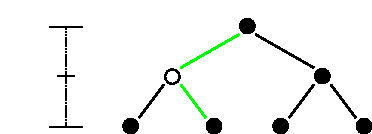
\includegraphics[width=\unitlength]{strmsum/figures/search.pdf}}%
    \put(-0.00356303,0.37186889){\color[rgb]{0,0,0}\makebox(0,0)[lt]{\begin{minipage}{1.32653733\unitlength}\raggedright Stream $\sentstream$ \end{minipage}}}%
    \put(0.05207008,0.30530006){\color[rgb]{0,0,0}\makebox(0,0)[lt]{\begin{minipage}{0.06721748\unitlength}\raggedright $\strmSent_1$\end{minipage}}}%
    \put(0.05326497,0.1819457){\color[rgb]{0,0,0}\makebox(0,0)[lt]{\begin{minipage}{0.06721748\unitlength}\raggedright $\strmSent_2$\end{minipage}}}%
    \put(0.05264783,0.04993889){\color[rgb]{0,0,0}\makebox(0,0)[lt]{\begin{minipage}{0.06721748\unitlength}\raggedright $\vdots$\end{minipage}}}%
    \put(0.483084,0.24693812){\color[rgb]{0,0,0}\rotatebox{27.31235445}{\makebox(0,0)[lt]{\begin{minipage}{0.18248248\unitlength}\raggedright \small extract\end{minipage}}}}%
    \put(0.76504897,0.29214953){\color[rgb]{0,0,0}\rotatebox{-29.99982322}{\makebox(0,0)[lt]{\begin{minipage}{0.13269863\unitlength}\raggedright \small skip\end{minipage}}}}%
  \end{picture}%
\endgroup%
  
  \caption{Search space for a stream of size two. The depth of the tree 
           corresponds to the position in the stream. Left branches indicate 
           extracting the current sentence as an update. Right branches skip 
           the current sentence. The path in green corresponds to one 
           trajectory through this space consisting of extracting sentence one, 
           then skipping sentence 2. The state represented by the hollow dot 
           corresponds to the stream at sentence position 2 with the update 
           summary containing sentence 1.}
  \label{fig:search}
\end{figure}

